\documentclass{article}

% set font encoding for PDFLaTeX, XeLaTeX, or LuaTeX
\usepackage{ifxetex,ifluatex}

\if\ifxetex T\else\ifluatex T\else F\fi\fi T%
  \usepackage{fontspec}
\else
  \usepackage[T1]{fontenc}
  \usepackage[utf8]{inputenc}
  \usepackage{lmodern}
\fi

\usepackage{amsmath}
\usepackage{amssymb}
\usepackage{amsthm}
\usepackage{mathtools}
\usepackage{physics}

\usepackage{enumitem}
\usepackage{multicol}
\usepackage{graphicx}
\usepackage{hyperref}
\usepackage[parfill]{parskip}
\usepackage{lipsum}
\usepackage[export]{adjustbox}

\usepackage{xparse} 
\usepackage{subfig} 
\usepackage{xparse} 
\usepackage{float}

\usepackage{biblatex} 

%%%%%This is an image table command, can likely be deleted
\newcommand{\subf}[2]{

%
{\small 
\begin{tabular}
  [t]{@{}c@{}} #1\ 
  \#2 
\end{tabular}
}

%
} 

\makeatletter
\renewcommand*\env@matrix[1][c]{\hskip -\arraycolsep
  \let\@ifnextchar\new@ifnextchar
  \array{*\c@MaxMatrixCols #1}}
\makeatother
%%%%%% Tensor Product
\NewDocumentCommand{\tens}{e{_^}}{ 
\mathbin{\mathop{\otimes}\displaylimits \IfValueT{#1}{_{#1}} \IfValueT{#2}{^{#2}} }}
%%%%%% Add \R Reals
\newcommand{\R}{\mathbb{R}} 
%%%%%% Add \theorem float
\newtheorem{theorem}{Theorem}
%%%%%% Add \definition float
\theoremstyle{definition} 
\newtheorem{definition}{Definition}[section]
%%%%%%%%%%%%%%%%%%%%%%%%%%%%%%%%%%%%%%%%%%%%%%%%%%%%%%%%%%%%%%%%%%%%%%%%%%%%%%%%%%%%%%%%%%%%%%%%%%%%%%%%%%%%%%%%%%%%%%%%%%
%%%%%Uncomment to add citation library 
\bibliography{lib} 
\title{Rubella Report}
\author{David Helekal, Yiping Zhang}

\begin{document}
\maketitle
\section{Model}

Let us define a $k$-age group compartmental SIRV model for the infection dynamics of the diseases covered by the MMR vaccine. This model takes the form of a system of four vectorised ordinary differential equations. Each of the $k$ vector entries then corresponds to a given age subgroup with span $m_i, \quad i\in1...k$. Each equation then governs the dynamics what proportion of the subpopulations is susceptible, infected, recovered, or has been vaccinated.

\begin{align*}
&\frac{d\mathbf{s}}{dt} &=&& \mathbf{B} - (\mathbf{V} - \mathbf{D})\mathbf{s} - \mathbf{s}*(\beta(t)\mathbf
{i})+\delta_{t_{end}}(t)\mathbf{M}\mathbf{s}\\
%%%%%%%%%%%%%%%%%%%%%%%%%%%%%%%%%%%%%%%%%%%%%%%%%%%%%%%%%%%%%%%%%%%%%%%%%%%%%%%%%%%%%%%%%%%%%%%%%%%%%%%%%%%%%%%%%%%%%%%%%%
&\frac{d\mathbf{i}}{dt} &=&&\mathbf{s}*(\beta(t)\mathbf
{i}) - (\mathbf{D}-\mathbf{d} - \mathbf{\gamma})\mathbf{i}+\delta_{t_{end}}(t)\mathbf{M}\mathbf{i}\\
%%%%%%%%%%%%%%%%%%%%%%%%%%%%%%%%%%%%%%%%%%%%%%%%%%%%%%%%%%%%%%%%%%%%%%%%%%%%%%%%%%%%%%%%%%%%%%%%%%%%%%%%%%%%%%%%%%%%%%%%%%
&\frac{d\mathbf{r}}{dt} &=&& \gamma\mathbf{i} - \mathbf{D}\mathbf{r}+\delta_{t_{end}}(t)\mathbf{M}\mathbf{r}\\
%%%%%%%%%%%%%%%%%%%%%%%%%%%%%%%%%%%%%%%%%%%%%%%%%%%%%%%%%%%%%%%%%%%%%%%%%%%%%%%%%%%%%%%%%%%%%%%%%%%%%%%%%%%%%%%%%%%%%%%%%%
&\frac{d\mathbf{v}}{dt} &=&& \mathbf{V}\mathbf{s}-\mathbf{D}\mathbf{v} +\delta_{t_{end}}(t)\mathbf{M}\mathbf{v}\\
%%%%%%%%%%%%%%%%%%%%%%%%%%%%%%%%%%%%%%%%%%%%%%%%%%%%%%%%%%%%%%%%%%%%%%%%%%%%%%%%%%%%%%%%%%%%%%%%%%%%%%%%%%%%%%%%%%%%%%%%%%
\end{align*}
$\mathbf{s}*\mathbf{i}\quad\textit{Denotes the elementwise product}$\\
Where:
\begin{align*}
&\mathbf{s}, \mathbf{i}, \mathbf{r} ,\mathbf{v}\in \mathbb{R}^k& \quad& \text{are k-age group classes of susceptible, infected, recovered}\\
%%%%%%%%%%%%%%%%%%%%%%%%%%%%%%%%%%%%%%%%%%%%%%%%%%%%%%%%%%%%%
%%%%%%%%%%%%%%%%%%%%%%%%%%%%%%%%%%%%%%%%%%%%%%%%%%%%%%%%%%%%%
&\mathbf{B} \in \mathbb{R}^{k\times k}, \mathbf{B}:=diag(B,0,...,0)& \quad& \text{Birth rate}\\
%%%%%%%%%%%%%%%%%%%%%%%%%%%%%%%%%%%%%%%%%%%%%%%%%%%%%%%%%%%%%
%%%%%%%%%%%%%%%%%%%%%%%%%%%%%%%%%%%%%%%%%%%%%%%%%%%%%%%%%%%%%
&\mathbf{V} \in \mathbb{R}^{k\times k}, \mathbf{V}:=diag(V_1,...,V_k) &\quad& \text{Vaccination rates}\\
%%%%%%%%%%%%%%%%%%%%%%%%%%%%%%%%%%%%%%%%%%%%%%%%%%%%%%%%%%%%%
%%%%%%%%%%%%%%%%%%%%%%%%%%%%%%%%%%%%%%%%%%%%%%%%%%%%%%%%%%%%%
&\mathbf{D} \in \mathbb{R}^{k\times k}, \mathbf{D}:=diag(D_1,...,D_k) &\quad& \text{Death rates due to other causes}\\
%%%%%%%%%%%%%%%%%%%%%%%%%%%%%%%%%%%%%%%%%%%%%%%%%%%%%%%%%%%%%
%%%%%%%%%%%%%%%%%%%%%%%%%%%%%%%%%%%%%%%%%%%%%%%%%%%%%%%%%%%%%
&\mathbf{d} \in \mathbb{R}^{k\times k}, \mathbf{d}:=diag(d_1,...,d_k) &\quad& \text{Death rates due to disease}\\
%%%%%%%%%%%%%%%%%%%%%%%%%%%%%%%%%%%%%%%%%%%%%%%%%%%%%%%%%%%%%%%%%%%%%%%%%%%%%%%%%%%%%%%%%%%%%%%%%%%%%%%%%%%%%%%%%%%%%%%%%%
&\beta(t):\mathbb{R} \rightarrow \mathbb{R}^{k\times k}&\quad& \text{The (potentially time-dependent) contact rate}\\
%%%%%%%%%%%%%%%%%%%%%%%%%%%%%%%%%%%%%%%%%%%%%%%%%%%%%%%%%%%%%
%%%%%%%%%%%%%%%%%%%%%%%%%%%%%%%%%%%%%%%%%%%%%%%%%%%%%%%%%%%%%
&\gamma \in \mathbb{R}&\quad&\text{Recovery rate}\\
%%%%%%%%%%%%%%%%%%%%%%%%%%%%%%%%%%%%%%%%%%%%%%%%%%%%%%%%%%%%%
%%%%%%%%%%%%%%%%%%%%%%%%%%%%%%%%%%%%%%%%%%%%%%%%%%%%%%%%%%%%%
&\mathbf{M}\in\mathbb{R}^{k\times k}&\quad& \text{The age group transition matrix}
\end{align*}

  where $\mathbf{M}$ has the structure
\begin{gather*}
\mathbf{M}=\begin{bmatrix}
-m_1^{-1} &      &        &        &    \\
 m_1^{-1} & -m_2^{-1} &        &        &    \\
     &  m_2^{-1} & -m_3^{-1}   &        &    \\
     &      & \ddots & \ddots &    \\
     &      &		 & m_{k-1}^{-1}& 0\\
\end{bmatrix}
\end{gather*}
\section{Data}
Epidemiologic age structured data for Rubella can be obtained from either Health Protection Agency archives \cite{agency_epidemiological_nodate} or from ECDC Atlas of Infectious Diseases \cite{noauthor_surveillance_nodate}.\\
Immunisation is available from the NHS COVER reports \cite{noauthor_childhood_nodate}.\\
As a starting point for contact rate matrices, the POLYMOD study \cite{mossong_social_2008} can utilised.\\
This data should enable us to parametrise and fit an age stratified SIRV model for years 1998-2019. Adding gender structure should be explored as well in the case of rubella as the primary concern is cogenital rubella syndrome in newborns. 
\center
\begin{figure}
  [h] 
  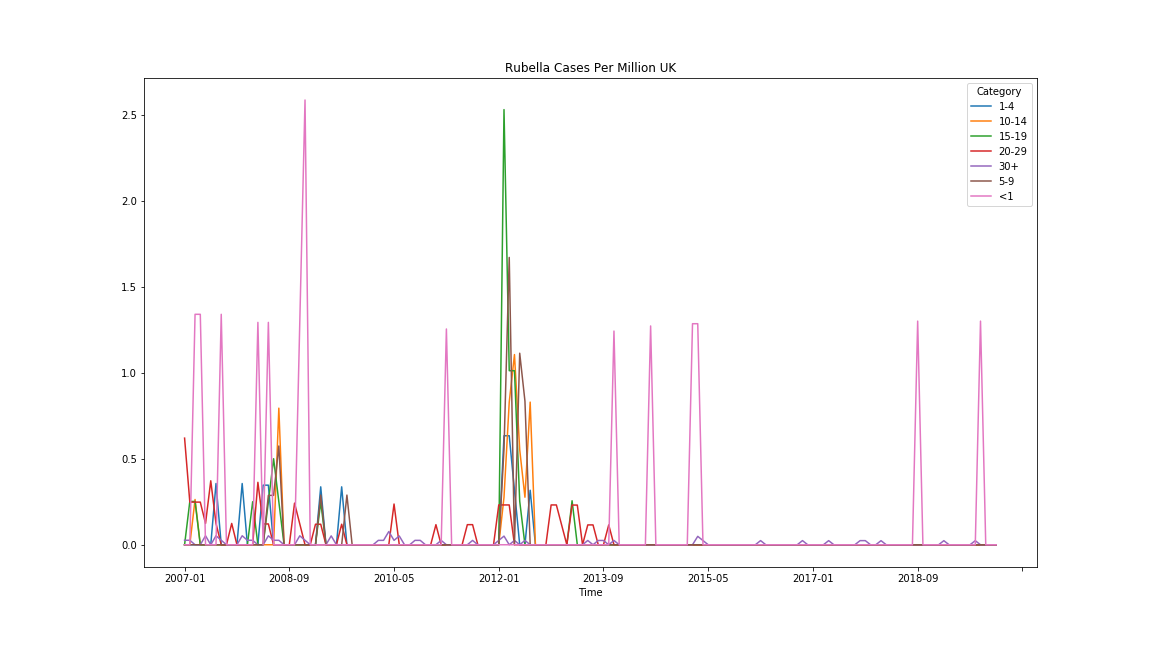
\includegraphics[width=1 
  \textwidth]{../data_nb/Rubella20072018}
  \caption{ECDC data for Rubella cases in the UK}
\end{figure}
\newpage
%%%%%should have a separate page for bibliography
\printbibliography  
\end{document}
